% === T17 - Planificación de Procesos ===
% David Alejandro Gonzalez Marquez
% fokerman@gmail.com
% https://github.com/fokerman/computingSystemsCourse

\documentclass[aspectratio=169]{beamer}
\usepackage{../packages}

\definecolor{nuevo}{HTML}{f8e45c}
\definecolor{preparado}{HTML}{f5c211}
\definecolor{ejecucion}{HTML}{ffa348}
\definecolor{terminado}{HTML}{c0bfbc}
\definecolor{espera}{HTML}{99c1f1}

\title{\Huge Planificación de Procesos\\ \emph{Scheduler}}
\author{David Alejandro González Márquez}
\institute{}

\date{}

\begin{document}

\begin{frame}[plain]
    \titlepage
    \begin{textblock}{100}(30,80)
    \begin{tcolorbox}[size=small,width=\textwidth,colback={gray!30},title={}]
    \begin{center}
     \scriptsize Clase disponible en: \url{https://github.com/fokerman/computingSystemsCourse}
    \end{center}
    \end{tcolorbox}
    \end{textblock}
%     \begin{textblock}{140}(10,70)
%     \textcolor{rojo}{
%     \textbf{Atención}: La clase será grabada por el anfitrión para su posterior y eventual uso académico dentro de nuestra institución. Su participación en la clase implica brindar su consentimiento para participar en la grabación, aunque pueden mantener su video apagado.}
%     \end{textblock}
\end{frame}

\begin{frame}{Planificador o \emph{Scheduler}}
    \small
    En un sistema donde múltiples procesos son ejecutados compartiendo tiempo de CPU,\\ debe existir un componente encargado de coordinar su uso.
    \pause
    \begin{center}
    \begin{tcolorbox}[size=small,width=0.85\textwidth,sharp corners,title={ \textcolor{naranjauca}{\emph{scheduler} o planificador} }]
    \small
    Componente del Sistema Operativo encargado de \textbf{coordinar} el uso del procesador o procesadores por los procesos en ejecución.
    Decide en que momento un proceso debe ser ejecutado y cuando su ejecución debe ser detenida.
    \end{tcolorbox}
    \end{center}
    \pause
    \bigskip
    La implementación del \emph{scheduler} es crítica para evaluar el desempeño de los Sistemas Operativos.\\
    \medskip
    Una gran parte del esfuerzo de optimización y captura de métricas tiene foco en el \emph{scheduler},\\
    sin embargo \textcolor{verdeuca}{\textbf{no existe un algoritmo de planificación perfecto.}}\\
    \medskip
    El desempeño de los \emph{scheduler} dependen del  \textcolor{verdeuca}{\textbf{\emph{workload} al que este expuesto el sistema.}}\\
\end{frame}

\begin{frame}[t]{Criterios para la planificación}
    \vspace{0.2cm}
    Los algoritmos de planificación miden su eficienta según los \textbf{objetivos que buscan optimizar}.\\
    \begin{textblock}{90}(10,22)
    \medskip \small
    \uncover<2->{ \textcolor{naranjauca}{\textbf{Tiempo de ejecución (turnaround)}}\\
    \hspace{0.5cm}Tiempo que demora un proceso en completar su ejecución.\\
    \vspace{0.3cm} }
    \uncover<3->{ \textcolor{naranjauca}{\textbf{Utilización de la CPU}}\\
    \hspace{0.5cm}Porcentaje de uso de la CPU.\\
    \vspace{0.3cm} }
    \uncover<4->{ \textcolor{naranjauca}{\textbf{Tiempo de respuesta}}\\
    \hspace{0.5cm}Tiempo percibido por el usuario en procesos interactivos.\\
    \vspace{0.3cm} }
    \uncover<5->{ \textcolor{naranjauca}{\textbf{Rendimiento (throughput)}}\\
    \hspace{0.5cm}La cantidad de procesos que se terminan por unidad de tiempo.\\
    \vspace{0.3cm} }
    \uncover<6->{ \textcolor{naranjauca}{\textbf{Tiempo de espera}}\\
    \hspace{0.5cm}Tiempo entre que el proceso está preparado y es ejecutado.\\
    \vspace{0.3cm} }
%     \uncover<7->{ \textcolor{naranjauca}{\textbf{Ecuanimidad (\emph{fairness})}}\\
%     \hspace{0.5cm}Todos los procesos reciben una cuota justa de tiempo de CPU.\\
%     \hspace{0.5cm}\textcolor{gray}{No necesariamente tiene que ser igual para todos los procesos.}\\
%     \vspace{0.1cm} }
%     \uncover<8->{ \textcolor{naranjauca}{\textbf{Liberación de recursos}}\\
%     \hspace{0.5cm}Priorizar la ejecución de procesos que más recursos consumen.\\
%     \hspace{0.5cm}\textcolor{gray}{(para que los liberen cuanto antes)}\\
%     \vspace{0.1cm} }
    \end{textblock}
    \begin{textblock}{52}(103,45)
    \uncover<7->{
    \begin{tcolorbox}[size=small,width=\textwidth,sharp corners,title={}] \small %\footnotesize
    Ahora, ¿Qué sucede sí un proceso conoce el criterio de planificación y busca aprovecharlo para usar más tiempo el CPU?\\
    \textcolor{gray}{Un \emph{malware} podría y el sistema debería detectarlo, ya que en caso contrario afectaría al resto de los procesos ejecutando en el sistema.}
    \end{tcolorbox} }
    \end{textblock}
\end{frame}

\begin{frame}[t]{Intercambio de procesos}
    El intercambio de procesos se puede dar bajo las siguientes situaciones:
    \begin{textblock}{80}(5,20) \small
    \begin{itemize}
    \setlength\itemsep{0.3cm}
    \item<2->[-] \textbf{desalojado: {\scriptsize \textcolor{ejecucion}{en ejecución} $\rightarrow$ \textcolor{preparado}{preparado} } }\\
    El proceso deja de ser ejecutado cuando\\ termina su tiempo asignado (\textcolor{verdeuca}{\textbf{\emph{quantum}}}).
    \item<2->[-] \textbf{pausado: {\scriptsize \textcolor{ejecucion}{en ejecución} $\rightarrow$ \textcolor{preparado}{preparado} } }\\
    El proceso deja de ser ejecutado producto\\ de una \textcolor{verdeuca}{\textbf{interrupción}}.
    \item<3->[-] \textbf{operación de E/S: {\scriptsize \textcolor{ejecucion}{en ejecución} $\rightarrow$ \textcolor{espera}{en espera} } }\\
    El proceso deja de ser ejecutado producto\\ de una \textcolor{verdeuca}{\textbf{solicitud de E/S}}.
    \item<4->[-] \textbf{salida: {\scriptsize \textcolor{ejecucion}{en ejecución} $\rightarrow$ \textcolor{terminado}{terminado} } }\\
    El proceso en ejecución \textcolor{verdeuca}{\textbf{termina}}.
    \end{itemize}
    \end{textblock}
    \begin{textblock}{100}(80,30) \only<2->{\includegraphics[scale=1.2]{img/estados_fixed-layer1.pdf}} \end{textblock}
\end{frame}

\begin{frame}{Tipos de planificación}
    \begin{textblock}{70}(10,22)
    \only<2->{\textcolor{naranjauca}{\textbf{Sin desalojo}} o \textcolor{naranjauca}{\textbf{Cooperativa}}\\ \vspace{0.2cm}
    El proceso solo puede dejar de ejecutar si termina, o realiza una operación de E/S.\\}
    \vspace{1.9cm}
    \only<3->{\textcolor{naranjauca}{\textbf{Con desalojo}} o \textcolor{naranjauca}{\textbf{Apropiativa}}\\ \vspace{0.2cm}
    El proceso puede dejar de ejecutar bajo cualquier condición, incluso si el planificador así lo decide.}
    \end{textblock}
    \begin{textblock}{100}(90,15) \only<2->{\includegraphics[scale=1]{img/estados_fixed-layer2.pdf}} \end{textblock}
    \begin{textblock}{100}(90,50) \only<3->{\includegraphics[scale=1]{img/estados_fixed-layer1.pdf}} \end{textblock}
\end{frame}

\begin{frame}{Comportamiento de los procesos}
    \begin{textblock}{140}(9,12)
    \uncover<1->{
    \small Para el planificador un proceso puede entenderse como secuencia intercalada de \textcolor{verdeuca}{\textbf{instrucciones}} y \textcolor{verdeuca}{\textbf{eventos de E/S}}.\\
    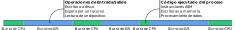
\includegraphics[scale=0.6]{img/burst_CPU_IO.pdf} }
    \end{textblock}
    \begin{textblock}{75}(9,45)
    \uncover<2->{
    \small Dependiendo del tipo de proceso, puede generar mayor o menor cantidad de eventos de entrada/salida.\\
    \medskip
    \textcolor{verdeuca}{La figura indica la distribución de tiempos entre que un proceso comienza a ser ejecutado hasta que realiza un evento de E/S.\\} }
    \end{textblock}
    \begin{textblock}{80}(90,42)
    \only<2->{ 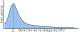
\includegraphics[scale=0.8]{img/burst.pdf} }
    \end{textblock}
    \begin{textblock}{145}(9,73)
    \uncover<3->{
    \small Las ráfagas o \emph{burst} de E/S suelen durar \textbf{mucho más tiempo}, que las ráfagas de CPU.\\
    \medskip
    \textcolor{naranjauca}{\textbf{Por esta razón los procesos están la mayor parte del tiempo esperando que finalicen operaciones de E/S.}} }
    \end{textblock}
\end{frame}

\begin{frame}{Tiempo de ráfaga}
    \small
    Cuando aparece un \textbf{nuevo proceso}, no tenemos información de cuanto tiempo va a demorar ejecutando.
    \begin{center}
    Entonces, \textcolor{naranjauca}{\textbf{¿Cómo podemos estimar el tiempo de ráfaga?}}
    \end{center}
    \pause
    \textcolor{verdeuca}{
    Una vez que ejecuta por primera vez, reportamos su tiempo de ráfaga.\\
    Predecimos a partir de ahí, el próximo tiempo de ráfaga en base a las ráfagas anteriores.\\}
    \medskip
    La estimación se realiza usando un promedio entre las ráfagas, dando mayor peso a las ráfagas más recientes y menor peso a las ráfagas más antiguas.\\
    \pause
    \begin{tcolorbox}[size=small,width=\textwidth,sharp corners,title={}] \small 
    En general se utiliza el \textbf{promedio exponencial} que se calcula como:
    \begin{center}
    { \large $\tau_{n+1} = \alpha \cdot t_n + (1 - \alpha) \cdot \tau_n$ }
    \end{center}
    \footnotesize
    Donde $t_n$ es el tiempo de ráfaga en el instante $n$, y $\tau_{n+1}$ es el tiempo de ráfaga estimado.\\
    El coficiente $\alpha$ regula la incidencia de las ráfagas anteriores en el cálculo.
    \end{tcolorbox}
    Para $\alpha = 0$ la última ráfaga no tiene ningún peso, mientras que para $\alpha = 1$ se considera solo la última.
    En general, se suele usar  $\alpha = 0.5$.    
\end{frame}

\begin{frame}{Algoritmos de planificación}
    Los algoritmos pueden ser muy variados, vamos a conocer algunos de estos,\\
    entendiendo funcionamiento, ventajas y desventajas.\\
    \bigskip
    \begin{itemize}
    \setlength\itemsep{0.15cm}
    \item[-] \textbf{First-come, first-served (FCFS)}
    \item[-] \textbf{Round Robin (RR)}
    \item[-] \textbf{Shortest Job First (SJF)}
    \item[-] \textbf{Shortest Remaining Time First (SRTF)}
    \item[-] \textbf{Priority Scheduling}
    \item[-] \textbf{Multilevel Queue Scheduling}
    \item[-] \textbf{Multilevel Feedback Queue Scheduling}
    \end{itemize}
    \bigskip
    \small
    \textcolor{gray}{Además, para ilustrar su funcionamiento vamos a construir \emph{diagramas de Gantt},
    indicando como cada algoritmo asigna procesos al CPU y calculando el tiempo promedio de espera para medir su eficiencia.}\\
\end{frame}

\begin{frame}{\large Algoritmos de planificación: \Large First-come, first-served (FCFS)}
    \begin{textblock}{85}(8,12)
    \uncover<1->{ \small
    Los procesos \textcolor{verdeuca}{\textbf{se ejecutan según el orden de llegada.}}
    Se trata de un algoritmo simple y \textbf{cooperativo}, ya que los procesos nunca son desalojados.\\ }
    \uncover<2->{ \medskip Se implementa utilizando una cola de procesos ordenados según su llegada. }
    \end{textblock}
    \begin{textblock}{50}(100,12)
    \only<3->{
    \textcolor{gray}{\small Ejemplo}\\ \vspace{-0.3cm}
    \textcolor{gray}{\rule{\linewidth}{0.8pt}}
    \begin{tabular}{C{1.2cm}|C{1.2cm}|C{1.2cm}}
    \small Proceso     & \scriptsize Tiempo de llegada & \scriptsize Tiempo de ráfaga \tiny (ms)\\ %\hline \hline
    \small \texttt{P1} & $0$               & $35$           \\
    \small \texttt{P2} & $0$               & $10$           \\
    \small \texttt{P3} & $0$               & $5$            \\
    \end{tabular} }
    \end{textblock}
    \begin{textblock}{100}(8,38) \only<4->{\includegraphics[scale=0.9]{img/schedulers-layer1.pdf}} \end{textblock} % FCFS
    \begin{textblock}{100}(8,38) \only<5->{\includegraphics[scale=0.9]{img/schedulers-layer2.pdf}} \end{textblock} % FCFS
    \begin{textblock}{100}(8,38) \only<6->{\includegraphics[scale=0.9]{img/schedulers-layer3.pdf}} \end{textblock} % FCFS
    \begin{textblock}{100}(8,38) \only<9->{\includegraphics[scale=0.9]{img/schedulers-layer4.pdf}} \end{textblock} % FCFS CS
    \begin{textblock}{140}(8,52) \small
    \uncover<7->{Tiempo de espera promedio = $\frac{0 + 35 + 45}{3}$ = $\frac{80}{3}$ = $26.66$ ms.\\}
    \end{textblock}
    \begin{textblock}{140}(10,60)
    \uncover<9->{
    \begin{tcolorbox}[size=small,width=\textwidth,sharp corners,title={}] \footnotesize
    \textbf{En los diagramas se ignora el tiempo de \emph{task switch}.}\\
    Este tiempo se debe considerar cada vez que se cambia de un proceso a otro.\\
    Los algoritmos de \emph{scheduling} lo hacen para reducir los tiempos muertos.
    \end{tcolorbox}
    \small Para el ejemplo, la cantidad de \emph{task switch} = $2$. }
    \end{textblock}
\end{frame}

\begin{frame}{\large Algoritmos de planificación: \Large First-come, first-served (FCFS)}
    \begin{textblock}{85}(8,12)
    \uncover<1->{ \small
    ¿Qué sucede si en el ejemplo anterior el orden de llegada de los procesos fuera a la inversa?\\}
    \end{textblock}
    \begin{textblock}{50}(100,12)
    \only<1->{
    \textcolor{gray}{\small Ejemplo}\\ \vspace{-0.3cm}
    \textcolor{gray}{\rule{\linewidth}{0.8pt}}
    \begin{tabular}{C{1.2cm}|C{1.2cm}|C{1.2cm}}
    \small Proceso     & \scriptsize Tiempo de llegada & \scriptsize Tiempo de ráfaga \tiny (ms)\\ %\hline \hline
    \small \texttt{P3} & $0$               & $5$            \\
    \small \texttt{P2} & $0$               & $10$           \\
    \small \texttt{P1} & $0$               & $35$           \\
    \end{tabular} }
    \end{textblock}
    \begin{textblock}{100}(8,23) \only<2->{\includegraphics[scale=0.9]{img/schedulers-layer5.pdf}} \end{textblock} % FCFS 2
    \begin{textblock}{100}(8,23) \only<3->{\includegraphics[scale=0.9]{img/schedulers-layer6.pdf}} \end{textblock} % FCFS 2
    \begin{textblock}{100}(8,23) \only<4->{\includegraphics[scale=0.9]{img/schedulers-layer7.pdf}} \end{textblock} % FCFS 2
%     \begin{textblock}{100}(8,23) \only<5->{\includegraphics[scale=0.9]{img/schedulers-layer8.pdf}} \end{textblock} % FCFS 2 CS
    \begin{textblock}{140}(8,36) \small
    \uncover<4->{Tiempo de espera promedio = $\frac{0 + 5 + 15}{3}$ = $\frac{20}{3}$ = $6.66$ ms.}
    \end{textblock}
    \begin{textblock}{140}(10,48)
    \uncover<5->{
    \small
    \texttt{FCFS} es un algoritmo muy simple de implementar y aprovecha la CPU al máximo,\\
    ya que los procesos no son desalojados. Evitando el \emph{overhead} del \emph{task switch}.\\
    \bigskip
    Por otro lado, un proceso largo puede tomar el procesador por mucho tiempo,\\
    demorando al resto de los procesos (\emph{efecto convoy}).\\
    \bigskip
    \textcolor{verdeuca}{Este efecto se ve en el ejemplo anterior para el proceso \texttt{P1}.} }
    \end{textblock}
\end{frame}

\begin{frame}{\large Algoritmos de planificación: \Large Round Robin (RR)}
    \begin{textblock}{95}(8,12)
    \uncover<1->{ \small
    Cada proceso tiene asignado un \textbf{quantum} (tiempo máximo que\\ puede correr).
    \textcolor{verdeuca}{\textbf{Cuando un proceso consume su \emph{quantum}, se lo\\ desaloja y se ejecuta el siguiente proceso.}}\\
    Algoritmo similar al \texttt{FCFS} pero con \textbf{desalojo}.\\}
    \uncover<2->{ \medskip Se implementa utilizando una lista circular que se recorre en orden.}
    \end{textblock}
    \begin{textblock}{50}(100,12)
    \only<3->{
    \textcolor{gray}{\small Ejemplo} \hspace{2cm} \scriptsize \emph{quantum = $10$}\\ \vspace{-0.2cm}
    \textcolor{gray}{\rule{\linewidth}{0.8pt}}
    \begin{tabular}{C{1.2cm}|C{1.2cm}|C{1.2cm}}
    \small Proceso     & \scriptsize Tiempo de llegada & \scriptsize Tiempo de ráfaga \tiny (ms)\\ %\hline \hline
    \texttt{P1} & $0$               & $25$             \\
    \texttt{P2} & $0$               & $20$             \\
    \texttt{P3} & $0$               & $5$              \\
    \end{tabular} }
    \end{textblock}
    \begin{textblock}{100}(8,40) \only<4->{\includegraphics[scale=0.9]{img/schedulers-layer9.pdf}} \end{textblock} % RR
    \begin{textblock}{100}(8,40) \only<5->{\includegraphics[scale=0.9]{img/schedulers-layer10.pdf}} \end{textblock} % RR
    \begin{textblock}{100}(8,40) \only<6->{\includegraphics[scale=0.9]{img/schedulers-layer11.pdf}} \end{textblock} % RR
    \begin{textblock}{100}(8,40) \only<7->{\includegraphics[scale=0.9]{img/schedulers-layer12.pdf}} \end{textblock} % RR
    \begin{textblock}{100}(8,40) \only<8->{\includegraphics[scale=0.9]{img/schedulers-layer13.pdf}} \end{textblock} % RR
    \begin{textblock}{100}(8,40) \only<9->{\includegraphics[scale=0.9]{img/schedulers-layer14.pdf}} \end{textblock} % RR
    \begin{textblock}{100}(8,40) \only<11->{\includegraphics[scale=0.9]{img/schedulers-layer15.pdf}} \end{textblock} % RR CS
    \begin{textblock}{140}(8,54) \small
    \uncover<10->{Tiempo de espera promedio = $\frac{((25-10)+(45-35)) + ((10-0)+(35-20)) + (20-0)}{3}$ = $\frac{25+25+20}{3}$ = $\frac{70}{3}$ = $23.33$ ms.\\}
    \medskip
    \uncover<12->{
    \begin{tcolorbox}[size=small,width=\textwidth,sharp corners,title={\footnotesize Duración de \emph{quantum}, ¿fijo o variable?}] \footnotesize
    \textbf{Si es muy corto}, gran parte del tiempo estará dedicado a planificar y a hacer cambios de contexto.\\
    \textbf{Si es muy largo}, degenera en FCFS, y se vuelve inadecuado para procesos interactivos.\\
    \scriptsize
    En la práctica se usan \emph{quantums} de entre $10$ y $100$ ms mientras que el cambio de contexto toma $10$ $\mu s$ (microsegundos).\\
    \textcolor{gray}{Es decir, un cambio de contexto equivale a $0.001$ \emph{quantums}.}
    \end{tcolorbox} }
    \end{textblock}
    \begin{textblock}{50}(100,44)
    \uncover<11->{\small Cantidad de \emph{task switch} = $5$.}
    \end{textblock}
\end{frame}

\begin{frame}{\large Algoritmos de planificación: \Large Shortest Job First (SJF)}
    \begin{textblock}{85}(8,15)
    \uncover<1->{ \small
    Se ordenan los procesos según su tiempo de ráfaga, \textcolor{verdeuca}{\textbf{se elige al proceso con la ráfaga de CPU más corta}}.
    Si tienen el mismo tiempo de ráfaga, se elige al que llego primero.}
    \end{textblock}
    \begin{textblock}{50}(100,12)
    \only<2->{
    \textcolor{gray}{\small Ejemplo}\\ \vspace{-0.3cm}
    \textcolor{gray}{\rule{\linewidth}{0.8pt}}
    \begin{tabular}{C{1.2cm}|C{1.2cm}|C{1.2cm}}
    \small Proceso     & \scriptsize Tiempo de llegada & \scriptsize Tiempo de ráfaga \tiny (ms) \\ %\hline \hline
    \texttt{P1} & $0$               & $10$             \\
    \texttt{P2} & $0$               & $3$              \\
    \texttt{P3} & $0$               & $30$             \\
    \texttt{P4} & $0$               & $4$              \\
    \texttt{P5} & $0$               & $3$              \\
    \end{tabular} }
    \end{textblock}
    \begin{textblock}{100}(8,32) \only<3->{\includegraphics[scale=0.9]{img/schedulers-layer16.pdf}} \end{textblock} % SJF
    \begin{textblock}{100}(8,32) \only<4->{\includegraphics[scale=0.9]{img/schedulers-layer17.pdf}} \end{textblock} % SJF
    \begin{textblock}{100}(8,32) \only<5->{\includegraphics[scale=0.9]{img/schedulers-layer18.pdf}} \end{textblock} % SJF
    \begin{textblock}{100}(8,32) \only<6->{\includegraphics[scale=0.9]{img/schedulers-layer19.pdf}} \end{textblock} % SJF
    \begin{textblock}{100}(8,32) \only<7->{\includegraphics[scale=0.9]{img/schedulers-layer20.pdf}} \end{textblock} % SJF
    \begin{textblock}{100}(8,32) \only<8->{\includegraphics[scale=0.9]{img/schedulers-layer21.pdf}} \end{textblock} % SJF CS
    \begin{textblock}{140}(8,46) \small
    \uncover<7->{Tiempo de espera promedio = $\frac{10 + 0 + 20 + 6 + 3}{5}$ = $\frac{39}{5}$ = $7.8$ ms.\\}
    \medskip
    \uncover<8->{\small Cantidad de \emph{task switch} = $4$.}
    \end{textblock}
    \begin{textblock}{140}(10,65)
    \only<9->{
    \begin{tcolorbox}[size=small,width=\textwidth,sharp corners,title={}] \small
    Este algoritmo es \textbf{óptimo} para minimiza el tiempo de espera promedio.\\
    Sin embargo, no lo es, ya que se cuenta con una predicción del tiempo de ráfaga de cada proceso.
    \end{tcolorbox}
    }
    \end{textblock}
\end{frame}

\begin{frame}{\large Algoritmos de planificación: \Large Shortest Remaining Time First (SRTF)}
    \begin{textblock}{85}(8,15)
    \uncover<1->{ \small
    Similar a \texttt{JSF} pero con \textbf{desalojo}.\\
    \textcolor{verdeuca}{\textbf{Se elige al proceso con la ráfaga de CPU más corta y se lo ejecuta hasta que su quantum termine}}. }
    \end{textblock}
    \begin{textblock}{50}(95,12)
    \only<2->{
    \textcolor{gray}{\small Ejemplo}\\ \vspace{-0.3cm}
    \textcolor{gray}{\rule{\linewidth}{0.8pt}}
    \begin{tabular}{C{1.2cm}|C{1.2cm}|C{1.2cm}l}
    \small Proceso     & \scriptsize Tiempo de llegada & \scriptsize Tiempo de ráfaga & \\ %\hline \hline
    \texttt{P1} & $0$               & $13$             & \hspace{-0.5cm} \scriptsize \only<2->{$\rightarrow$ 13} \hspace{0.1cm} \only<3->{3}  \hspace{0.1cm} \only<4->{0}\\
    \texttt{P2} & $2$               & $8$              & \hspace{-0.5cm} \scriptsize \only<2->{$\rightarrow$}  \only<3->{8}  \hspace{0.1cm} \only<6->{0}\\
    \texttt{P3} & $12$              & $4$              & \hspace{-0.5cm} \scriptsize \only<2->{$\rightarrow$}  \only<4->{4}  \hspace{0.1cm} \only<5->{0}\\
    \texttt{P4} & $20$              & $18$             & \hspace{-0.5cm} \scriptsize \only<2->{$\rightarrow$}  \only<6->{18} \hspace{0.1cm} \only<7->{8} \hspace{0.1cm} \only<9->{0}\\
    \texttt{P5} & $30$              & $7$              & \hspace{-0.5cm} \scriptsize \only<2->{$\rightarrow$}  \only<7->{7}  \hspace{0.1cm} \only<8->{0}\\
    \end{tabular} }
    \end{textblock}
    \begin{textblock}{100}(8,33) \only<3->{\includegraphics[scale=0.9]{img/schedulers-layer22.pdf}} \end{textblock} % SRTF 10
    \begin{textblock}{100}(8,33) \only<4->{\includegraphics[scale=0.9]{img/schedulers-layer23.pdf}} \end{textblock} % SRTF 3
    \begin{textblock}{100}(8,33) \only<5->{\includegraphics[scale=0.9]{img/schedulers-layer24.pdf}} \end{textblock} % SRTF 4
    \begin{textblock}{100}(8,33) \only<6->{\includegraphics[scale=0.9]{img/schedulers-layer25.pdf}} \end{textblock} % SRTF 8
    \begin{textblock}{100}(8,33) \only<7->{\includegraphics[scale=0.9]{img/schedulers-layer26.pdf}} \end{textblock} % SRTF 10
    \begin{textblock}{100}(8,33) \only<8->{\includegraphics[scale=0.9]{img/schedulers-layer27.pdf}} \end{textblock} % SRTF 7
    \begin{textblock}{100}(8,33) \only<9->{\includegraphics[scale=0.9]{img/schedulers-layer28.pdf}} \end{textblock} % SRTF 8
    \begin{textblock}{100}(8,33) \only<10->{\includegraphics[scale=0.9]{img/schedulers-layer29.pdf}} \end{textblock} % SRTF CS        
    \begin{textblock}{140}(8,50) \small
    \uncover<9->{Tiempo de espera promedio =\\
    \vspace{0.2cm}
    = $\frac{0 + (17-2) + (13-12) + ((25-20)+(42-35)) + (35-30)}{5}$ = $\frac{0 + 15 + 1 + (5+7) + 5}{5}$ = $\frac{33}{5}$= $6.6$ ms.\\}
    \medskip
    \uncover<10->{\small Cantidad de \emph{task switch} = $5$.}
    \end{textblock}
    \begin{textblock}{140}(8,72)
    \only<11->{\small
    Este algoritmo también es conocido como \emph{Shortest Time to Completion (STCF)} 
    }
    \end{textblock}
\end{frame}

\begin{frame}[t]{\large Algoritmos de planificación: \Large Priority Scheduling}
    \small
    Se define un criterio de prioridad entre procesos, \textcolor{verdeuca}{\textbf{los procesos de prioridad más alta, ejecutarán antes que los procesos de prioridad más baja}}.\\
    \pause
    \bigskip
    Los criterios de prioridad pueden ser:
    \begin{itemize}
     \item[-] \textcolor{naranjauca}{Internos}: Se toman medidas y en base a estas se asigna una prioridad. (Ej: \texttt{SJF})
     \item[-] \textcolor{naranjauca}{Externos}: Se asigna una prioridad en base al usuario o alguna característica del proceso.
    \end{itemize}
    \pause
    \bigskip
    \begin{tcolorbox}[size=small,width=\textwidth,sharp corners,title={}]
    La aplicación de prioridades se puede combinar con otros algoritmos de planificación,\\ ya sean cooperativos como apropiativos.
    \end{tcolorbox}
    \pause
    \bigskip
    Asignar una prioridad arbitraria a los procesos puede generar \textbf{inanición} (\textbf{\emph{starvation}}).\\
    \textcolor{verdeuca}{Es decir, un proceso de baja prioridad queda esperando indefinidamente tiempo de CPU.}\\
    \medskip
    \pause
    Para evitar este problema se aplican criterios de \textbf{envejecimiento}.\\
    \textcolor{verdeuca}{A medida que aumenta el tiempo de espera, se aumenta la prioridad del proceso.}
\end{frame}

\begin{frame}{\large Algoritmos de planificación: \Large Multilevel Queue Scheduling}
    \begin{textblock}{80}(10,15)
    \small
    \uncover<1->{
    En un planificador de colas multinivel, los procesos son \textbf{separados en distintas colas} según su tipo o prioridad.\\
    \bigskip
    Cada cola utilizará su \textbf{propio algoritmo de planificación} para elegir el próximo proceso a ejecutar.\\
    }
    \bigskip
    \uncover<2->{
    Además se debe elegir la cola sobre la cual tomar procesos.\\
    \textcolor{verdeuca}{\textbf{Este algoritmo suele ser de prioridades fijas y apropiativo.\\}}
    \medskip
    { \footnotesize \textcolor{gray}{Es decir, hasta que las colas de mayor prioridad no tengan procesos, 
    no se puede ejecutar un procesos de una cola de menor prioridad, 
    y si llega un proceso de una cola de mayor prioridad este debe ser ejecutado.}\\ }
    \bigskip
    }
    \uncover<3->{
    El esquema resultante es \textbf{poco flexible}\\ y no es libre de \textbf{inanición}.
    }
    \end{textblock}
    \begin{textblock}{100}(100,20)
    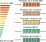
\includegraphics[scale=1]{img/multilevel_queue.pdf}
    \end{textblock}
\end{frame}

\begin{frame}{\large Algoritmos de planificación: \Large Multilevel Feedback Queue Scheduling}
    \begin{textblock}{80}(10,15)
    \small
    En este esquema los procesos se pueden \textbf{mover} entre las distintas colas de prioridades.\\
    \medskip
    \uncover<2->{
    Existirá una relación entre la prioridad de un proceso y el tiempo que tiene asignado para su \emph{quantum}.\\
    { \footnotesize \textcolor{verdeuca}{Procesos de mayor prioridad tendrán menor \emph{quantum}, mientras que procesos de menor prioridad tendrán un \emph{quantum} mayor. } }\\
    }
    \medskip
    \uncover<3->{
    Cuando un proceso consume todo su \emph{quantum}, se lo pasa a una cola de menor prioridad, es decir mayor \emph{quantum}.\\
    \medskip
    { \footnotesize \textcolor{gray}{ Podemos generar \textbf{inanición}, ya que siempre se ejecutan los procesos de mayor prioridad.
    Para evitar este problema los procesos que pasen mucho tiempo en las colas de menor prioridad, se los mueve a colas de mayor prioridad.} }\\
    }
    \medskip
    \uncover<4->{
    El esquema resulta más flexible y resuelve los problemas de las colas multinivel.
    }
    \end{textblock}
    \begin{textblock}{100}(100,20)
    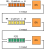
\includegraphics[scale=1]{img/multilevel_feedback_queue.pdf}\\
    \vspace{0.5cm}
    \tiny
    \uncover<2->{
    Procesos de \textbf{ráfagas cortas} $\rightarrow$ en colas de \textbf{mayor prioridad}.\\
    Procesos de \textbf{ráfagas largas} $\rightarrow$ en colas de \textbf{menor prioridad}.\\
    Procesos de \textbf{ráfagas irregulares} $\rightarrow$ se moverán entre las colas.\\
    }
    \end{textblock}
\end{frame}

\begin{frame}{Algoritmos de Planificación}
    Para diseñar algoritmos de planificación se utilizan \textbf{modelos de \emph{workloads}} de uso de sistemas.\\
    \medskip \pause
    Estos modelos se basan en \textbf{datos reales} y buscan reflejar la complejidad de todo un conjunto de procesos ejecutando en un sistema.\\
    \medskip \pause
    En la práctica, los diseñadores de Sistemas Operativos \textbf{modifican variables de configuración} de sus \emph{scheduler} para adaptarse a la evolución de los \emph{workloads}.\\
    \bigskip \pause
    \textcolor{verdeuca}{\textbf{Los \emph{schedulers} de los Sistemas Operativos en general no administran procesos, sino \emph{threads}.}}\\
    \medskip \pause
    Además tienen en cuenta en su planificación: el uso de la \textbf{memoria} (\emph{memory stall}),\\
    el \textbf{balanceo de la carga} de los procesadores (\emph{overloaded}), la \textbf{afinidad} con un determinado procesador (\emph{cache}), y el \textbf{tipo} de procesador (\emph{big.little}) entre otras características.
\end{frame}

\begin{frame}[fragile]
    \frametitle{Bibliografía}
    \begin{itemize}
        \setlength\itemsep{0.5cm}
        \item[-] \small Silberschatz, ``Fundamentos de Sistemas Operativos'', 7ma Edición, 2006.\\
        \begin{itemize}
            \item \textbf{Capítulo 5 - Planificación de la CPU}, páginas 137-151 y 161-165
        \end{itemize}
        \item[-] \small Tanenbaum, ``Modern Operating Systems'', 4th Edition, 2015.\\
        \begin{itemize}
            \item \textbf{Chapter 2 - Processes and Threads}
            \begin{itemize}
                \item 2.4 Scheduling - Páginas 149-165
            \end{itemize}
        \end{itemize}
    \end{itemize}
\end{frame}

\begin{frame}[fragile]
    \frametitle{Ejercicios}
    \vfill
    Con lo visto, ya pueden resolver todos los ejercicios de la Guía de Planificación de procesos.
    \vfill
\end{frame}

\begin{frame}[plain]
    \begin{center}
    \vspace{2cm}
    \huge ¡Gracias!\\
    \vspace{2cm}
    \normalsize Recuerden leer los comentarios adjuntos\\ en cada clase por aclaraciones.
    \end{center}
\end{frame}

\end{document}

